\documentclass[11pt,a4paper]{ivoa}
\input tthdefs
\usepackage{tabulary}  % for nicer tables

\title{Workshop (pre)Conclusions}

% see ivoatexDoc for what group names to use here
\ivoagroup{Data Model}

\author{Laurent Michel}
\author{Jesus Salgado}

\editor{Laurent Michel}

% \previousversion[????URL????]{????Concise Document Label????}
\previousversion{This is the first public release}
       

\begin{document}
\begin{abstract}
This note summarises the work done on the use-cases and give the preliminary conclusions that must lead a common strategy for improving interoperability with VO models.
\end{abstract}


\section*{Acknowledgments}

We thank all contributors who implemented the use cases or participated in discussions. 
We also thank the speakers who presented their views as developers or data providers.

\section*{Conformance-related definitions}

The \emph{Virtual Observatory (VO)} is a
general term for a collection of federated resources that can be used
to conduct astronomical research, education, and outreach.
The \href{https://www.ivoa.net}{International
Virtual Observatory Alliance (IVOA)} is a global
collaboration of separately funded projects to develop standards and
infrastructure that enable VO applications.

\section{Introduction}

The data model workshop has been initiated by the TCG in November 2020.
It is a 4 steps process that must issue a global strategy for the model usage in the VO; this means sharing a common way to get a better interoperability by mapping data on VO models .

\begin{figure}
\centering

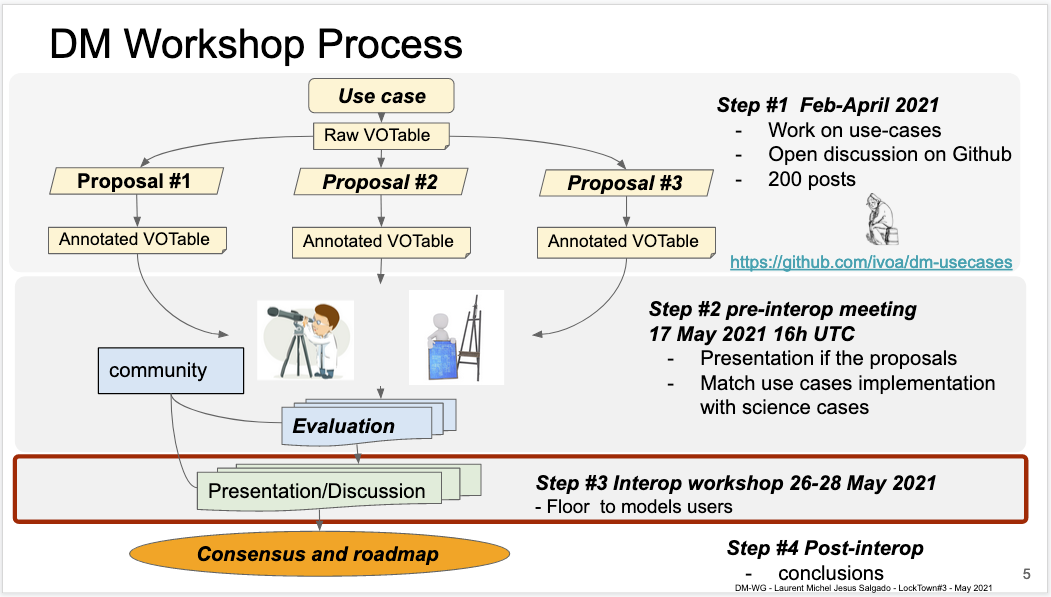
\includegraphics[width=0.9\textwidth]{fig1.png}
\caption{DM workshop}
\label{fig:workshop}
\end{figure}

The primary goal of this workshop was to answer the following questions

\begin{itemize}
\item Do the proposed models cover the science use-cases?
\item What is the best mapping strategy?
\item What is the most suitable annotation syntax.?
\end{itemize}

If we get a positive answer to all of the 3 questions, we will be able to propose a strait way to annotate data.
Any other information can be retrieved in the Github repository (https://github.com/ivoa/dm-usecases).

\section{Tools and Models}
\subsection{Models}

\begin{itemize}
\item \textbf{Coords (PR)} describes values associated with their coordinate systems.
\item \textbf{Meas (PR)} describes measures as Coord instances associated with errors.
\item \textbf{PhotDM (REC)} describes photometry filters, photometric systems, magnitude systems, zero
points etc.
\item \textbf{DataSet (WD)} Describes the structure and
content of generic Dataset metadata for the IVOA.
\item \textbf{CubeDM  (WD)}  presents an abstracted representation of NDimensional
cube datasets.
\item \textbf{Mango (WD)}  proposes a flexible way to expose data related to astronomical
source objects in an interoperable way.
\end{itemize}

In addition to this 2 ad-hoc models have been used:
\begin{itemize}
\item A model based on MANGO components for the complex time series (F. Bonnarel et al.).
\item Model classes referring to Meas/Coord elements but with different structures (M. Demleitner).
\end{itemize}

\subsection{Mapping Syntax}

The final solution should be complete enough to
allow a proper object mapping but simple enough to be implemented. 
Two different syntaxes have been used to annotate the use-cases datasets.

\begin{itemize}
\item \textbf{VODML Mapping (WD)} proposed by G. Lemson et al. in 2018.
\item \textbf{ModelInstanceInVot (WD)} proposed by L. michel et al. in 2020.
\end{itemize}

It is to be noted that ModelInstanceInVot derives from VODML Mapping.

\subsection{Clients APIs}

All the tools are still in prototype phase as they are not implementing
an agreed standard mapping. Once the IVOA mapping  approach is defined, IVOA implementors should 
collaborate to convert the library in a reference reusable implementation. This is an open issue on finding implementors
resources from IVOA members

\begin{itemize}
\item \textbf{Astropy extension (Markus Demleitner)}  designed to process the annotation as proposed by Markus Demleitner.
\item \textbf{Rama (Mark. C. Dittmar et al.)} Python API based on generated code designed to process  VODML Mapping annotations in connection with Astropy.
\item \textbf{modelinstanceinvot-code (L. Michel et al.)} Python API based on dictionaries designed to process ModelInstanceInVot annotations in connection with PyVO.
\item \textbf{AWK scripts (Mireille Louys)} shell script showing that ModelInstanceInVot annotations  can be read with basic shell scripts.
\end{itemize}


\section{Use Case Implementation}
\subsection{Use Cases}

5 use-cases on 10 have been selected to assess the conclusions. This choice covers most of the current science cases. 
Table \ref{tbl:use-case} gives a brief description of them. All details can be found on Github.

\begin{table}[!htbp]
\small
\centering
\begin{tabulary}{\linewidth}{|c|J|}       
       \hline 
            \textbf{Case} & 
            \textbf {Purpose}\\
       \hline         \hline  
            time series & identifying the whole thing as a time series, 
                                  \newline  Identifying the independent axis/axes, associating values and errors 
                                  \newline Figuring out the observation position  
                                  \newline This use-case comes with one simple time-series  and 2 more complex one (Gaia  and ZTF) where photometric points are mixed in data tables\\
       \hline 
            standard properties  & 
            Allow clients to easily retrieve  scientifically relevant source properties \\
       \hline 
            combined data & 
            Aggregation of various pieces of information into a single VOTable \\
       \hline 
            precise astrometry & 
            Client authors want to recognise all information in catalogues relevant to precision astrometry 
            \newline(e.g., distances or radial velocities as necessary in foreshortening calculations) \\
        \hline 
            column grouping & 
            The data table must be annotated in a way that a client can easily detect column groups. 
            \newline These groups have no particular semantic. They are just telling that the measures are related each to other.\\
      \hline 
     \end{tabulary}
     \caption{Use-cases selection} 
     \label{tbl:use-case}
 \end{table}

\subsection{Implementation}

Matrix \ref{tbl:implementation} gives an implementation overview. All details can be found in the Github repository.

\begin{table}[!htbp]
\small
\centering
\begin{tabulary}{\linewidth}{|c|J|J|J|J|J|J|J|}       
       \hline 
            {\small \textbf{Case} }& 
           {\tiny \textbf{MD.AS} } & 
           {\tiny  \textbf{C.VM} } & 
            {\tiny \textbf{C.MIV} } & 
           {\tiny  \textbf{FB.MIV} } & 
            {\tiny \textbf{M.VM}  } & 
            {\tiny \textbf{M.MIV} } &
            {\tiny \textbf{V.OF} }\\
       \hline         \hline  
           simple time series &
           X&
           X&
           X&
            &
            &
            &
            \\
      \hline 
           Gaia time series &
           X&
           &
           X&
           X&
            &
            &
           \\
      \hline 
           ZTF time series &
           X&
           &
           X&
           X &
            &
            &
           \\
      \hline 
           std properties &
           &
           &
           &
           &
           X &
           X &
           X 
           \\
      \hline 
           combined data &
           &
           &
           &
           &
           X &
           X
            \\
      \hline 
           precise astrometry &
           X &
           &
           &
           &
           &
           X 
           \\
      \hline 
           column grouping &
           &
           &
           &
           &
           X &
           X &
           X \\
      \hline 
     \end{tabulary}
     \caption{Implementation matrix (MD: M. Demleitner, C: CubeDM, FB: F.Bonnarel, M: Mango, AS: annotation scheme, VM: VODML mapping, MIV: ModelInstanceInVot, V: Vizier, OF: On the fly) } 
     \label{tbl:implementation}
 \end{table}

\section{Requirements}

The main requirement shared by all the stakeholders is not to break existing things but to add missing features.
There is no strong demand for working with data mapped on models, but there is a real interest to use this mechanism 
to fill some gaps and to implement new functions.

\subsection{Science Requirements}

\begin{itemize}
\item VOTable annotations APIs must be included in AstroPy or PyVo,
\item Need for making multi-body data (asteroids, planets...) interoperable
\item Need for a standard for multi-messenger meta-data
\item Need for a model for photon lists
\item Need for an accurate time model for moving objects
\item Need for a model for orbital information
\item Need for a better support for X-ray data (photon based datasets, source-detection or spectrum-model association, probabilistic errors)
\end{itemize}

\subsection{Data Provider Requirements}

\begin{itemize}
\item Need for adding data provenance
\item Need for grouping measures
\item Need for a better description of the photometric calibrations
\item Need for a data annotation validator
\item Need simple views on complex models
\item On the fly annotation requires stable building blocks
\end{itemize}

\subsection{Client Developer Requirements}

\begin{itemize}
\item Data annotation must not come in replacement of existing processing but it must 
         add features that are currently missing such as a better coordinate systems or axis descriptions.
\item Need for a full spectrum characterisation.
\item VOTable annotations must come with reusable libraries at least in Java/Python
\end{itemize}
 
 
 \section{Conclusions}
 
 It has been decided before Interop to withdraw the approach consisting in mapping data on a set on independent model components and hence to keep working with integrated models re-using Meas/Coordinates/PhotDM classes.
 
\subsection{What Worked Very Well}

\begin{itemize}
\item Data contained in all 5 use-cases can be modelled with existing models
\item The 2 annotation syntaxes have been used with success
\item All  APIs have been able to process all annotations.
\item  It has been demonstrated that Enabling AstroPy or PyVo to work with annotated data is feasible without breaking the regular data access.
\end{itemize}

\subsection{What Has to Be Improved}

\begin{itemize}
\item The connection of PhotDM with Meas/Coordinate/Mango/Cube has to be tuned. This is a pending issue while the PhotDM VODML/XML has not be released.
\item Some update of Meas/Coordinate have been suggested, especially for the sky positions (see RFC2 page).
\item Some class rearrangements have been proposed in the MANGO Parameters.
\end{itemize}

\subsection{What Has to Be Discussed}

\begin{itemize}
\item It is very desirable to finally have one syntax. There are ongoing discussions to merge both proposals 
\item Model extensions to cover new use cases
\end{itemize}


\end{document}
